\let\negmedspace\undefined
\let\negthickspace\undefined
\documentclass{article}
\usepackage{cite}
\usepackage{amsmath,amssymb,amsfonts,amsthm}
\usepackage{algorithmic}
\usepackage{graphicx}
\usepackage{textcomp}
\usepackage{xcolor}
\usepackage{txfonts}
\usepackage{listings}
\usepackage{enumitem}
\usepackage{mathtools}
\usepackage{gensymb}
\usepackage{tfrupee}
\usepackage[breaklinks=true]{hyperref}
\usepackage{tkz-euclide} % loads  TikZ and tkz-base
\usepackage{listings}
%\usepackage{gvv}
%
%\usepackage{setspace}
%\usepackage{gensymb}
%\doublespacing
%\singlespacing

%\usepackage{graphicx}
%\usepackage{amssymb}
%\usepackage{relsize}
%\usepackage[cmex10]{amsmath}
%\usepackage{amsthm}
%\interdisplaylinepenalty=2500
%\savesymbol{iint}
%\usepackage{txfonts}
%\restoresymbol{TXF}{iint}
%\usepackage{wasysym}
%\usepackage{amsthm}
%\usepackage{iithtlc}
%\usepackage{mathrsfs}
%\usepackage{txfonts}
%\usepackage{stfloats}
%\usepackage{bm}
%\usepackage{cite}
%\usepackage{cases}
%\usepackage{subfig}
%\usepackage{xtab}
%\usepackage{longtable}
%\usepackage{multirow}
%\usepackage{algorithm}
%\usepackage{algpseudocode}
%\usepackage{enumitem}
%\usepackage{mathtools}
%\usepackage{tikz}
%\usepackage{circuitikz}
%\usepackage{verbatim}
%\usepackage{tfrupee}
%\usepackage{stmaryrd}
%\usetkzobj{all}
%    \usepackage{color}                                            %%
%    \usepackage{array}                                            %%
%    \usepackage{longtable}                                        %%
%    \usepackage{calc}                                             %%
%    \usepackage{multirow}                                         %%
%    \usepackage{hhline}                                           %%
%    \usepackage{ifthen}                                           %%
  %optionally (for landscape tables embedded in another document): %%
%    \usepackage{lscape}     
%\usepackage{multicol}
%\usepackage{chngcntr}
%\usepackage{enumerate}

%\usepackage{wasysym}
%\documentclass[conference]{IEEEtran}
%\IEEEoverridecommandlockouts
% The preceding line is only needed to identify funding in the first footnote. If that is unneeded, please comment it out.

\newtheorem{theorem}{Theorem}[section]
\newtheorem{problem}{Problem}
\newtheorem{proposition}{Proposition}[section]
\newtheorem{lemma}{Lemma}[section]
\newtheorem{corollary}[theorem]{Corollary}
\newtheorem{example}{Example}[section]
\newtheorem{definition}[problem]{Definition}
%\newtheorem{thm}{Theorem}[section] 
%\newtheorem{defn}[thm]{Definition}
%\newtheorem{algorithm}{Algorithm}[section]
%\newtheorem{cor}{Corollary}
\newcommand{\BEQA}{\begin{eqnarray}}
\newcommand{\EEQA}{\end{eqnarray}}
\newcommand{\define}{\stackrel{\triangle}{=}}
\theoremstyle{remark}
\newtheorem{rem}{Remark}

%\bibliographystyle{ieeetr}
\begin{document}
\title{LATEX ASSIGNMENT}
\author{ANAND}
\date{22-08-2023}
\maketitle
\section*{EXERCISE 10.3.7}
\begin{enumerate}
\item The ages of two friends ani and Biju differ  by $3$  years. Ani's father dharam is twice as old as Ani and Biju is twice as old as sister cathy. The ages of cathy and dharam differ by $30$ years. Find the ages of Ani and Biju.
\item  One says, \textquotedblleft Give me a hundred, Friend !  I shall then become twice as rich as you \textquotedblright. The other \textquotedblleft  if you give me ten, i shall be six times as rich as you \textquotedblright.  Tell me What is the amount of their (respective) capital? [From the bijaganita of bhaskara II] 
\\ $[Hint: X+100=2(y-100), y+10=6(x-10)]$
\item A train Covered a certain distance at a uniform speed. If the train would have been $10km/h$ faster, it would have taken $2$ hours less than the scheduled time. And, if the train were slower by 10km/h; it would have taken $3$ hours more than the scheduled time. Find the distance covered by the train.
\item The students of a class are made to stand in rows. If 3 Students are extra in a row, there would be $1$ row less. If $3$ students are less in a row, there would be $2$ rows more. Find the number of stuents in the class.
\item In a $\triangle ABC, \angle C=3 \angle B=2(\angle A+\angle B)$. Find the three angles
\item Draw the graphs of the equations $5x-y=5$ and $3x-y=3$. Determine the Co-ordinates of the vertices of the triangle formed by these lines and the $y$ axis.
\item Solve the following pair of linear equations;
\begin{enumerate}
\item
\begin{align}
px+qy=p-q\\ qx-py=p+q
\end{align}
\item
\begin{align}                                                   
ax+by=c\\ bx+ay=1+c
\end{align}
\item 
\begin{align}
\frac {x}{a}-\frac{y}{b}=0\\ ax+by=a^2+b^2
\end{align}
\item
\begin{align}
(a-b)x+(a+b)y=a^2-2ab-b^2\\ (a+b)(x+y)=a^2+b^2
\end{align}
\item
\begin{align}
152x-378y=-74\\ -378x+152y=-604
\end{align}
\end{enumerate}
\item $ABCD$ is a cyclic quadrilateral [see Fig. \ref{fig:3.7}]. Find the angles of the cyclic quadrilateral.
\begin{figure}[ht]
\centering
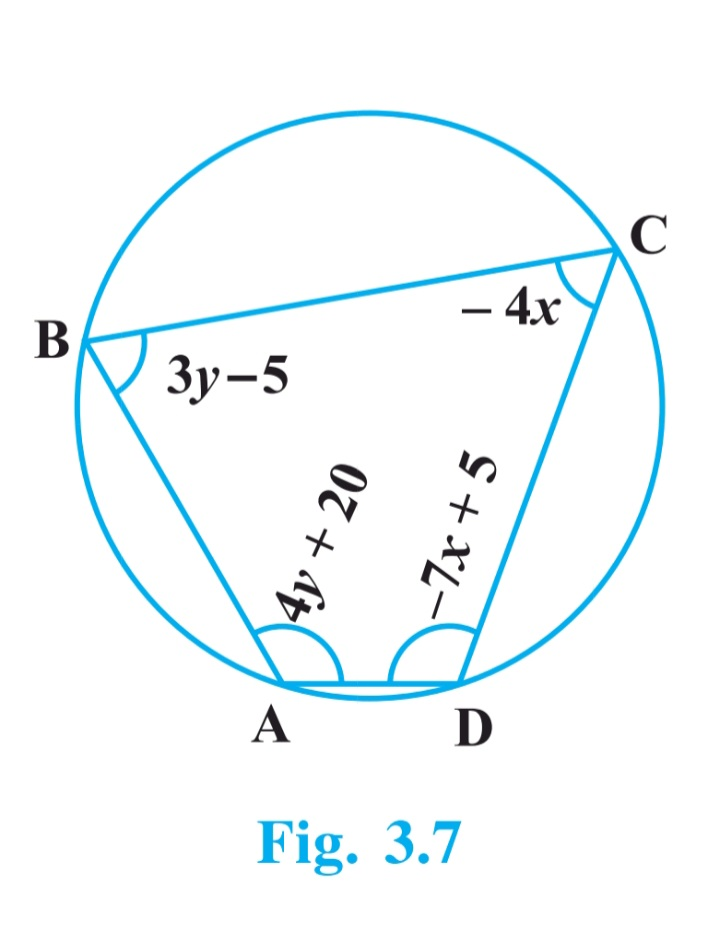
\includegraphics[width=\columnwidth]{figs/3.7.png}
\caption{3.7}
  \label{fig:3.7}
\end{figure}
\end{enumerate}
\end{document}  
